\documentclass[tikz,border=10pt]{standalone}
\usepackage{pgfplots}
\pgfplotsset{compat=1.18}
\begin{document}
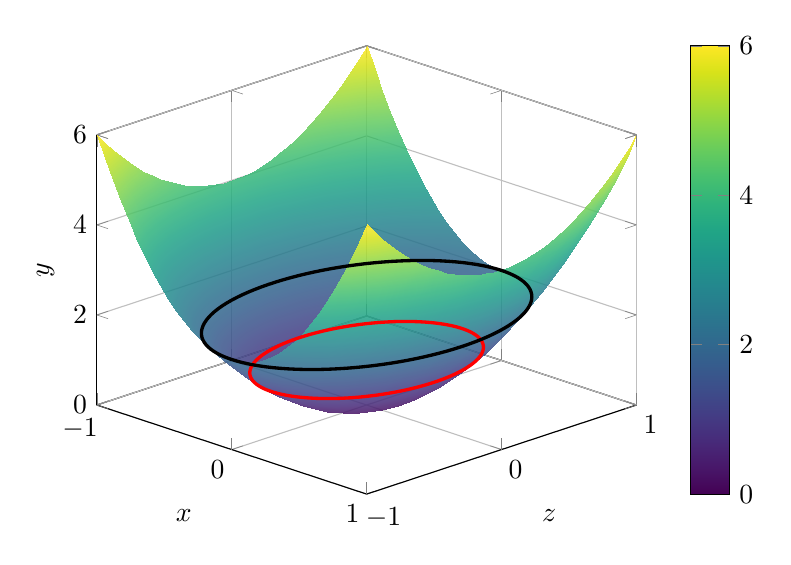
\begin{tikzpicture}
\begin{axis}[
    xlabel={$x$}, ylabel={$z$}, zlabel={$y$},
    view={45}{25},
    domain=-1:1, y domain=-1:1,
    samples=35, samples y=35,
    xmin=-1, xmax=1, ymin=-1, ymax=1, zmin=0, zmax=6,
    colormap/viridis,
    colorbar,
    grid=major
]
\addplot3[surf, shader=interp, opacity=0.85] {4*x^2 + 2*y^2};
\addplot3[red, very thick, domain=0:360, samples=120]
    ({sqrt(1/4)*cos(x)}, {sqrt(1/2)*sin(x)}, {1});
\addplot3[black, very thick, domain=0:360, samples=120]
    ({sqrt(2/4)*cos(x)}, {sqrt(2/2)*sin(x)}, {2});
\end{axis}
\end{tikzpicture}
\end{document}